\section{Программный пакет \texttt{NuPropagator}}

\texttt{NuPropagator}~\cite{nupropagator2022} — модуль для моделирования распространения потоков нейтрино через вещество, в частности сквозь Землю, с учётом взаимодействий с обменом $W$ и $Z$ бозонами. 
ПО \texttt{NuPropagator} реализована на языке \texttt{Python~3} и распространяется через платформу \texttt{PyPI}, обеспечивая простую установку и интеграцию в существующие симуляционные цепочки.

Структура ПО \texttt{NuPropagator} представлена на рис.~\ref{fig:nupropagator1}, на котором приведены соответствующие вспомогательные модули.
\begin{figure}[!h]
\centering
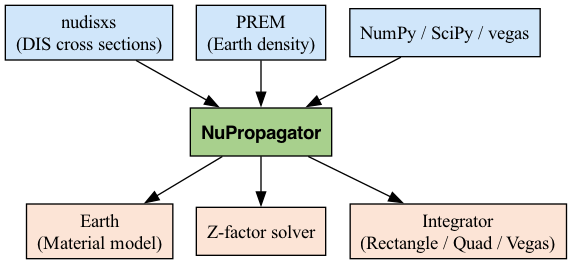
\includegraphics[width=\linewidth]{images/nupropagator_diagram.png}
\caption{Структура программного пакета \texttt{NuPropagator} и его зависимости.}
\label{fig:nupropagator1}
\end{figure}

В расчётах используются сечения взаимодействия нейтрино с нуклонами, предоставляемые пакетом \texttt{nudisxs}, модель плотности Земли PREM и итерационный метод $\mathcal{Z}$-фактора, описывающий эволюцию нейтринного спектра при прохождении через вещество. 
Такой подход позволяет учитывать как поглощение, так и регенерацию потоков за счёт нейтрального тока.

\texttt{NuPropagator} может использоваться как самостоятельный инструмент или как часть общего фреймворка, например, \texttt{NTSim}, разработанного для нейтринного телескопа Baikal-GVD~\cite{ntsim2025}. 
Он взаимодействует с генераторами событий, моделями детектора и другими компонентами цепочки симуляции, обеспечивая единое моделирование распространения нейтрино от источника до регистрации.
